\section{A Problem Class with Linear Physical Elements\label{sec:ch8:class}}

\newcommand{\xarch}{^{(i)}}
\newcommand{\xclass}{^{\mathcal{P}}}

%----------------------------------------------
\subsection{Linear Physical Elements\label{sec:ch8:linearelements}}

A useful framework for describing linear physical elements is bond graph modeling with power port nodes (or simply power nodes) \cite{Borutzky2010a}.
Power nodes are characterized by constitutive parameters and follow some constitutive relation (typically a fundamental physical law).
They can be classified as source nodes (\xcolor{Se}, \xcolor{Sf}), storage nodes (\xcolor{C}, \xcolor{I}),  resistive nodes (\xcolor{R}), reversible transducers (\xcolor{TF}, \xcolor{GY}), and junction nodes (\xcolor{0}, \xcolor{1}).
Some analogies for these power nodes in different energy domains are in Table~\ref{tb:ch8:analogies}.
An example of a \xcolor{TF} (transformer) is a lever, gear, or hydraulic cylinder.
The \xcolor{GY} (gyrator) typically describes the conversion between energy domains, such as with an electrical DC motor or mass accelerometer.
The \xcolor{0}-junction is analogous to Kirchhoff's current law and the \xcolor{1}-junction is analogous to the voltage law in electrical systems.
For more details on bond graph modeling, see Refs.~\cite{Borutzky2010a,Kypuros2013a, Karnopp2012a}

\begin{table}
\centering
\begin{tabular}{cccc}
\hline \hline
& \multicolumn{2}{c}{Linear Mechanical} & \\
Label & Intuitive & Topology Preserving & Electrical \\
\hline
\xcolor{Se} & Force & Velocity & Voltage  \\
\xcolor{Sf} & Velocity & Force & Current \\
\xcolor{C} & $1/K$ & $M$ & $C$  \\
\xcolor{I} & $M$ & $1/K$ & $I$ \\
\xcolor{R} & $B$ & $1/B$ & $R$ \\
\hline \hline
\end{tabular}
\caption{Some bond graph modeling analogies.\label{tb:ch8:analogies}}
\end{table}

The key property for systems represented by bond graphs with \glsfoo[noindex]{LTI} elements is that the equations of motion can be represented as a linear descriptor model.
If we denote the set of all constitutive parameters for a particular bond graph as \gls{parameters}, the model is of the form:
\begin{align}
\gls{dynE}(\bm{p}) \dot{\glsfoo[noindex]{timederiv}\gls{states}} = \gls{dynA}(\bm{p}) \bm{\xi} + \gls{dynB}(\bm{p}) \gls{sources}
\end{align} 

\noindent where $\bm{\xi}$ are the states and $\bm{s}$ are the sources.
The matrix $\bm{E}$ is invertible if there are no algebraic loops in the system \cite{Gonzalez2008a, Borutzky2010a}.
Here we assume that all algebraic loops are appropriately removed (e.g.,~see Ref.~\cite{Gonzalez2008a}) so that we have an explicit first-order \glsfoo[noindex]{ODE} with only $\{\bm{A}, \bm{B}\}$.

% new paragraph
The architecture design decisions will include what power nodes to include in the system and their connections.
The constitutive parameters will be the plant design variables (but the plant design could consist of more realistic variables such as the geometry of spring with a mapping back to the appropriate constitutive parameter).
The control decisions will come in the form of certain source types.
The sources may also be used to add various disturbances to the system.

%----------------------------------------------
\subsection{Problem Class Definition}

We would like to solve architecture design problems of the following form:
\begin{subequations}
\label{eq:ch8:levela}
\begin{align}
\min_{\gls{x}_{\glsfoo[noindex]{architecture}}} \quad & \gls{objective}_a(\bm{x}_a) + \Psi_{\gls{design}}\left( \gls{f}_{\glsfoo[noindex]{plant}}(\bm{x}_a), f_{\glsfoo[noindex]{control}}(\bm{x}_a) \right) \\
\text{subject to:} \quad & f_a(\bm{x}_a) = a \in \gls{feasible}_a
\end{align}
\end{subequations}

\noindent where $\bm{x}_a$ represents architecture design variables, $f_a(\bm{x}_a)$ is a mapping between the architecture design variables and the architecture $a$, and $\mathcal{F}_a$ is the feasible set of architectures.
$\Psi_a$ is the architecture-only objective function (such as a complexity metric that counts the number of additional components \cite{manuscript-pm-circuits}), while $\Psi_d$ is the general design objective function that includes dependence on the plant and control design.
This dependence is represented by the mapping functions $f_p$ and $f_c$ between the architecture and the plant $\bm{x}_p$ and \glsfoo[noindex]{OLC} \gls{olc} design variables. 

% new paragraph
A fair comparison between architecture candidates requires knowledge of the best possible performance for each candidate architecture.
To determine the value of $\Psi_d$ we must solve a suitable co-design problem.
This problem has the following form:
\begin{subequations}
\label{eq:ch8:codesign}
\begin{align}
\min_{\bm{x}_p^{\glsfirst{iarchitecture}}, \bm{u}\xarch} \quad & \Psi_d = \int_{\gls{time}_{\glsfoo[noindex]{initial}}}^{t_{\glsfoo[noindex]{final}}} \gls{lagrange}^{\glsfirst{class}}\left(t, \gls{output}, \bm{x}_p\xarch \right) dt + \gls{mayer}\xclass\left( \bm{y}(t_0), \bm{y}(t_f), \bm{x}_p\xarch \right) \\
\text{subject to:} \quad & \left[ \dot{\bm{\xi}} = \bm{f}\xclass\left( t, \bm{\xi}, \bm{u}, \bm{x}_p \right) \right]\xarch \\
& \gls{equality}\xclass\left(t, \bm{y}, \bm{x}_p\xarch \right) = \bm{0} \\
& \gls{inequality}\xclass\left(t, \bm{y}, \bm{x}_p\xarch \right) \leq \bm{0} \\
\text{where:} \quad & \bm{y} = \bm{y}\xclass\left( t, \bm{\xi}\xarch, \bm{u}\xarch, \bm{x}_p\xarch \right)
\end{align}
\end{subequations}

\noindent where $\Box\xarch$ indicates a problem formulation element appropriate for the $i$th candidate architecture from Prob.~(\ref{eq:ch8:levela}), $t$ is the time continuum between $t_0$ and $t_f$, and $\bm{y}$ are the (architecture-independent) outputs.
The problem elements $\{\mathcal{L}, \mathcal{M}, \bm{f}, \bm{h}, \bm{g} \}$ represent the Lagrange term, Mayer term, dynamics, equality constraints, and inequality constraints.

% new paragraph
The subscript \gls{problemclass} indicates a particular problem class that the problem elements must be in.
Here we will consider a class whose specific structure can lead to efficient solution strategies, but still covers the combined architecture, plant, and control design problems of interest.
Consider a function, $f\xclass$, in the problem class $\mathcal{P}$ with type $f$ (e.g.,~the type might be Lagrange term or inequality constraints).
Then $f\xclass$ must be a function where for fixed values of $\bm{x}_p\xarch$, $f\xclass$ has an equivalent \glsfoo[noindex]{LQDO} problem element described in Chapter~\ref{ch:5}.
With this specification of $\mathcal{P}$, Prob.~(\ref{eq:ch8:codesign}) is a strong candidate for the nested co-design solution strategy for the reasons discussed in Chapter~\ref{ch:3}, namely an efficient inner-loop strategy for LQDO.
This leads to the following trilevel solution approach.

%----------------------------------------------
\subsection{A Trilevel Solution Approach}

\begin{figure}
\centering
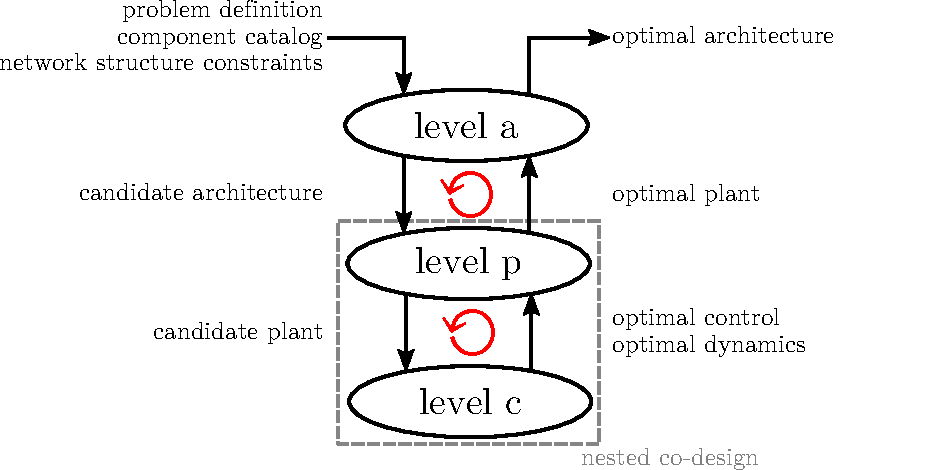
\includegraphics[scale=0.8]{../ch8/figures/trilevel}
\caption{The proposed trilevel solution strategy for combined architecture, plant, and control design.\label{fig:ch8:trilevel}}
\end{figure}

The trilevel solution approach used here is illustrated in Fig.~\ref{fig:ch8:trilevel}.
Each one of the three levels is now described.

\subsubsection{Architecture Design: Level a}

The topmost level is responsible for taking the problem definition, a user-defined component catalog, and network structure constraints and providing candidate architectures for the other levels.
Many architectures can be represented by colored graphs as the nodes in this representation scheme can be used to represent a variety of concepts. 
Therefore, the approach used here will be the perfect matching-based algorithm for generating all architectures in Chapter~\ref{ch:2}.
The different labels in the graphs will correspond to the power nodes in Sec.~\ref{sec:ch8:linearelements}.

\subsubsection{Plant Design: Level p}

The next level takes the candidate architecture and performs the outer-loop co-design tasks for the plant design \cite{Herber2017b}.
The appropriate optimization problem needs to be automatically created and solved.
Since these types of problems can be highly nonconvex (see Chapter~\ref{ch:3}), global search algorithms are utilized to help improve the confidence of finding the true optimal solution (in this chapter, a multistart approach is used, but an alternative is a genetic algorithm \cite{Papalambros2017a, Marti2003a, Eiben2003a}).

% new paragraph
An automated model generation procedure (see Sec.~\ref{sec:ch1:modelgen}) was developed to take the generated graphs and produce the appropriate (linear) model.
This procedure utilizes the \textsc{Simulink}/\textsc{Simscape} modeling environment to generate the appropriate diagram.
Each time a plant variable is updated, the model is regenerated through a linearization procedure.
This is a relatively expensive operation; a better method would generate an analytical representation of $\bm{A}(\bm{x}_p)$ and the other matrices so that it only needs to be performed once per candidate architecture.
Generating these equations is a task for future work.

\subsubsection{Control Design: Level c}

The deepest level takes the candidate plant and model to formulates the appropriate LQDO problem in Chapter~\ref{ch:5} \cite{manuscript-dt-qp}.
The structured-based description makes it relatively straightforward to handle a varying number of states and controls along with the output definitions.
Since this inner-loop co-design problem has a special structure, it can be solved with low computational expense and is guaranteed to be the global optimal control \cite{Herber2017b}.
We also note that the number of times level c is solved is much greater than level p, which is much greater than level a.